\section{Nanotecnologie}

	La nanotecnologia è un ramo della scienza applicata e della tecnologia che si occupa del controllo della materia su scala dimensionale nell'ordine del nanometro e della progettazione e realizzazione di dispositivi in tale scala.
	
	La nascita di questa nuova branca della tecnologia ci pone subito di fronte ad alcuni rischi, quali effetti avversi sulla salute umana o sull'ambiente in seguito ad un'esposizione volontaria o accidentale e la potenziale proprietà esplosiva delle nanostrutture.
	Risulta molto difficile fare una valutazione dei rischi associati a questa tecnologia per diversi fattori,
	in primo luogo c'è bisogno di personale specializzato e apparecchiature sofisticate;
	risulta poi difficile prevedere come determinate particelle si comporteranno una volta ingerite o disperse nell'ambiente; infine bisogna valutare la potenziale presenza di sostanze tossiche e la loro persistenza all'interno del corso o in natura.
	
	Al momento sono attive due grosse aree di ricerca: \emph{Electromagnetic Nano Communication} e \emph{comunicazione molecolare}.
	Nella comunicazione molecolare (\emph{molecular communication}) l'informazione è codificata all'interno di DNA, proteine, peptidi, etc ed è trasmessa per diffusione o trasporto attivo\footnote{Il trasporto attivo è il trasporto di molecole attraverso la membrana plasmatica mediato da una proteina transmembrana detta trasportatore di membrana.
		A differenza di quanto avviene nel trasporto passivo, nel trasporto attivo è richiesta una spesa energetica ed è sempre necessaria la mediazione di un trasportatore.
		In questa forma di trasporto le molecole si muovono contro un gradiente elettrico, chimico o elettrochimico.}.
	
	Nella comunicazione elettromagnetica si viene invece a creare una BAN (Body Area Network), composta da molti sensori che comunicano con un micro-gateway (tramite frequenze nell'ordine del THz).
	
	\paragraph{Information Centric Network (ICN)}
	Con l'aumento smisurato della mole di dati prodotta e scambiata attraverso la rete non è più possibile sfruttare una connessione di tipo host-to-host come si è fatto fino ad ora con IP (\emph{host centric network}), bisogna evolvere verso una \emph{information centric network} in cui la rete è in grado di immagazzinare i dati prodotti e fornirli a chi ne faccia richiesta successivamente; si parla così di \emph{in-network caching}.
	In una rete orientata al dato non collego più direttamente mittente e destinatario ma interrogo la rete e aspetto che qualcuno mi fornisca una risposta, sempre che questa non sia già stata inviata e sia quindi già presente.
	Chiunque ascolti la richiesta e sia in possesso di una valida copia del dato può rispondere;
	il dato restituito è firmato e opzionalmente anche criptato, così che la sua integrità ed associazione con il nome possano essere verificate.
	Si genera una \emph{disallocazione spaziale e temporale} del dato, tutto ciò di cui ho bisogno è il nome del contenuto a cui sono interessato.
	Le Figure \ref{fig:ICNdisegno} e \ref{fig:panoramicaICN} riportano uno schema di funzionamento di una ICN e una panoramica dei vantaggi offerti.
	
	Secondo lo schema della rete internet tradizionale le applicazioni erano orientate ai servizi offerti da alcuni server, una connessione di tipo host-to-host era quindi preferibile per l'interazione client-server.
	Al giorno d'oggi la rete internet risulta sensibilmente cresciuta rispetto a cinquant'anni fa, si parla di circa un miliardo di dispositivi attivi, di un trilione di pagine web indicizzate e annualmente vengono prodotti dati nell'ordine degli exabyte ($10^{18}$ Byte).
	Di fronte a una tale mole di dati IP mostra alcune criticità: necessita di Content Distribution Network
	\footnote{Content Delivery Network o Content Distribution Network (in sigla, CDN), ovvero \emph{Rete per la consegna di contenuti}, descrive un sistema di computer collegati in rete attraverso Internet sotto forma di sistema distribuito per ripartire contenuti (specialmente contenuti multimediali di grandi dimensioni in termini di banda, come l'IPTV) agli utenti finali ed erogare servizi di streaming audio e video.
	Grazie alla CDN si riducono notevolmente i tempi di caricamento di una pagina perché quando un contenuto viene richiesto, a rispondere è il server più vicino geograficamente e ciò si ripercuote positivamente sulle prestazioni del sito.}
	(CDN), offre un limitato supporto alla mobilità, basa la sicurezza sulla protezione degli host invece della protezione dei contenuti, non supporta il multicast su larga scala.
	
	\begin{figure}
		\centering
		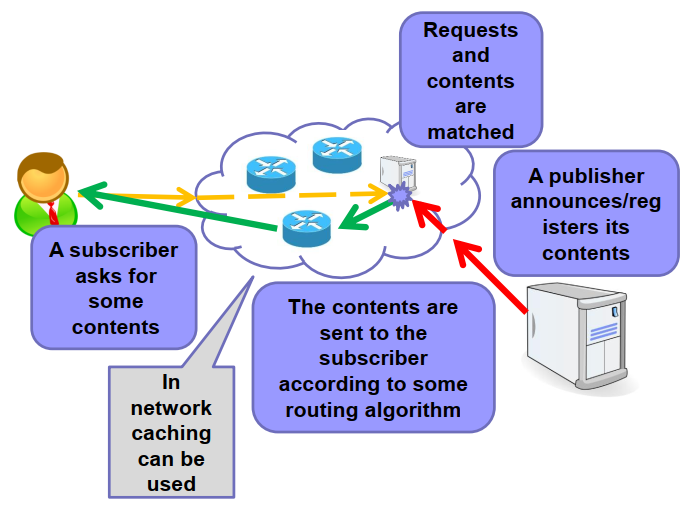
\includegraphics[width=0.6\textwidth]{lez8/ICNdisegno.png}
		\caption{Schema di una ICN}
		\label{fig:ICNdisegno}
	\end{figure}

	\begin{figure}
		\centering
		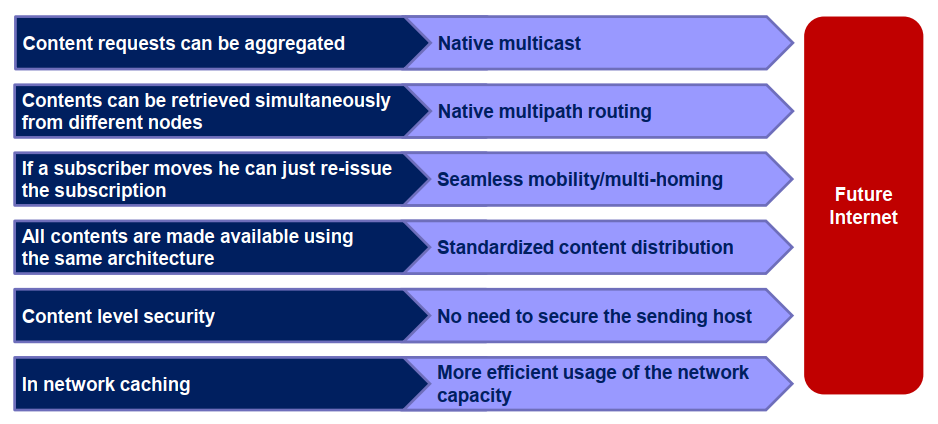
\includegraphics[width=0.9\textwidth]{lez8/futureInternet.png}
		\caption{panoramica delle caratteristiche e dei vantaggi offerti dalle ICN}
		\label{fig:panoramicaICN}
	\end{figure}

	\begin{figure}
		\centering
		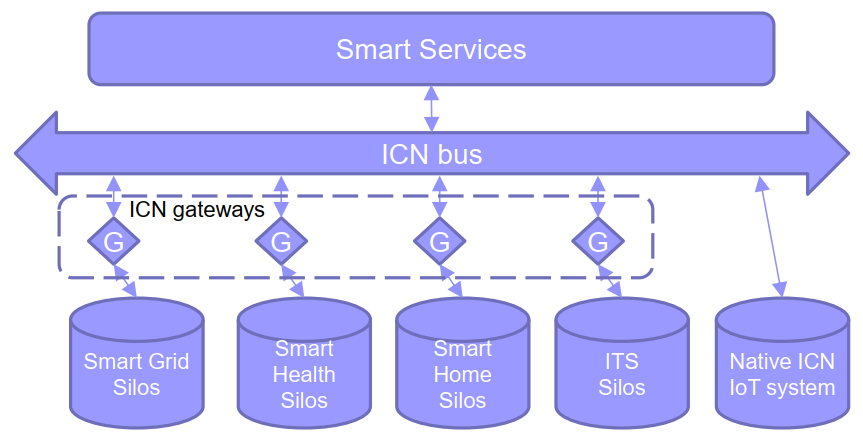
\includegraphics[width=0.6\textwidth]{lez8/ICN-iot-bigPicture.png}
		\caption{schema generale di un'architettura ICN-IoT}
		\label{fig:ICN-bigPicture}
	\end{figure}

	\begin{figure}
		\centering
		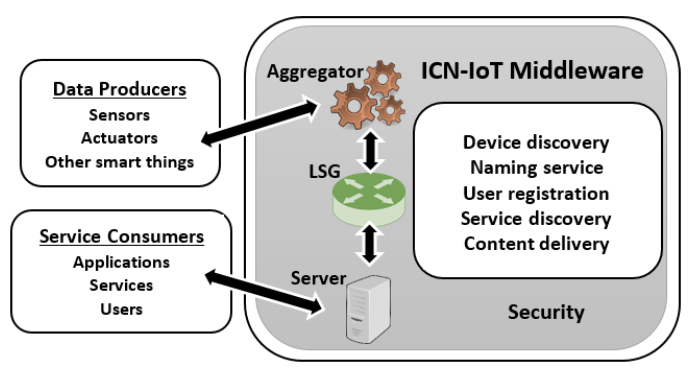
\includegraphics[width=0.7\textwidth]{lez8/ICN-iot-middleware.png}
		\caption{ICN-IoT middleware}
		\label{fig:ICN-middleware}
	\end{figure}


	